\begin{figure*}[thb!]
  \centering
  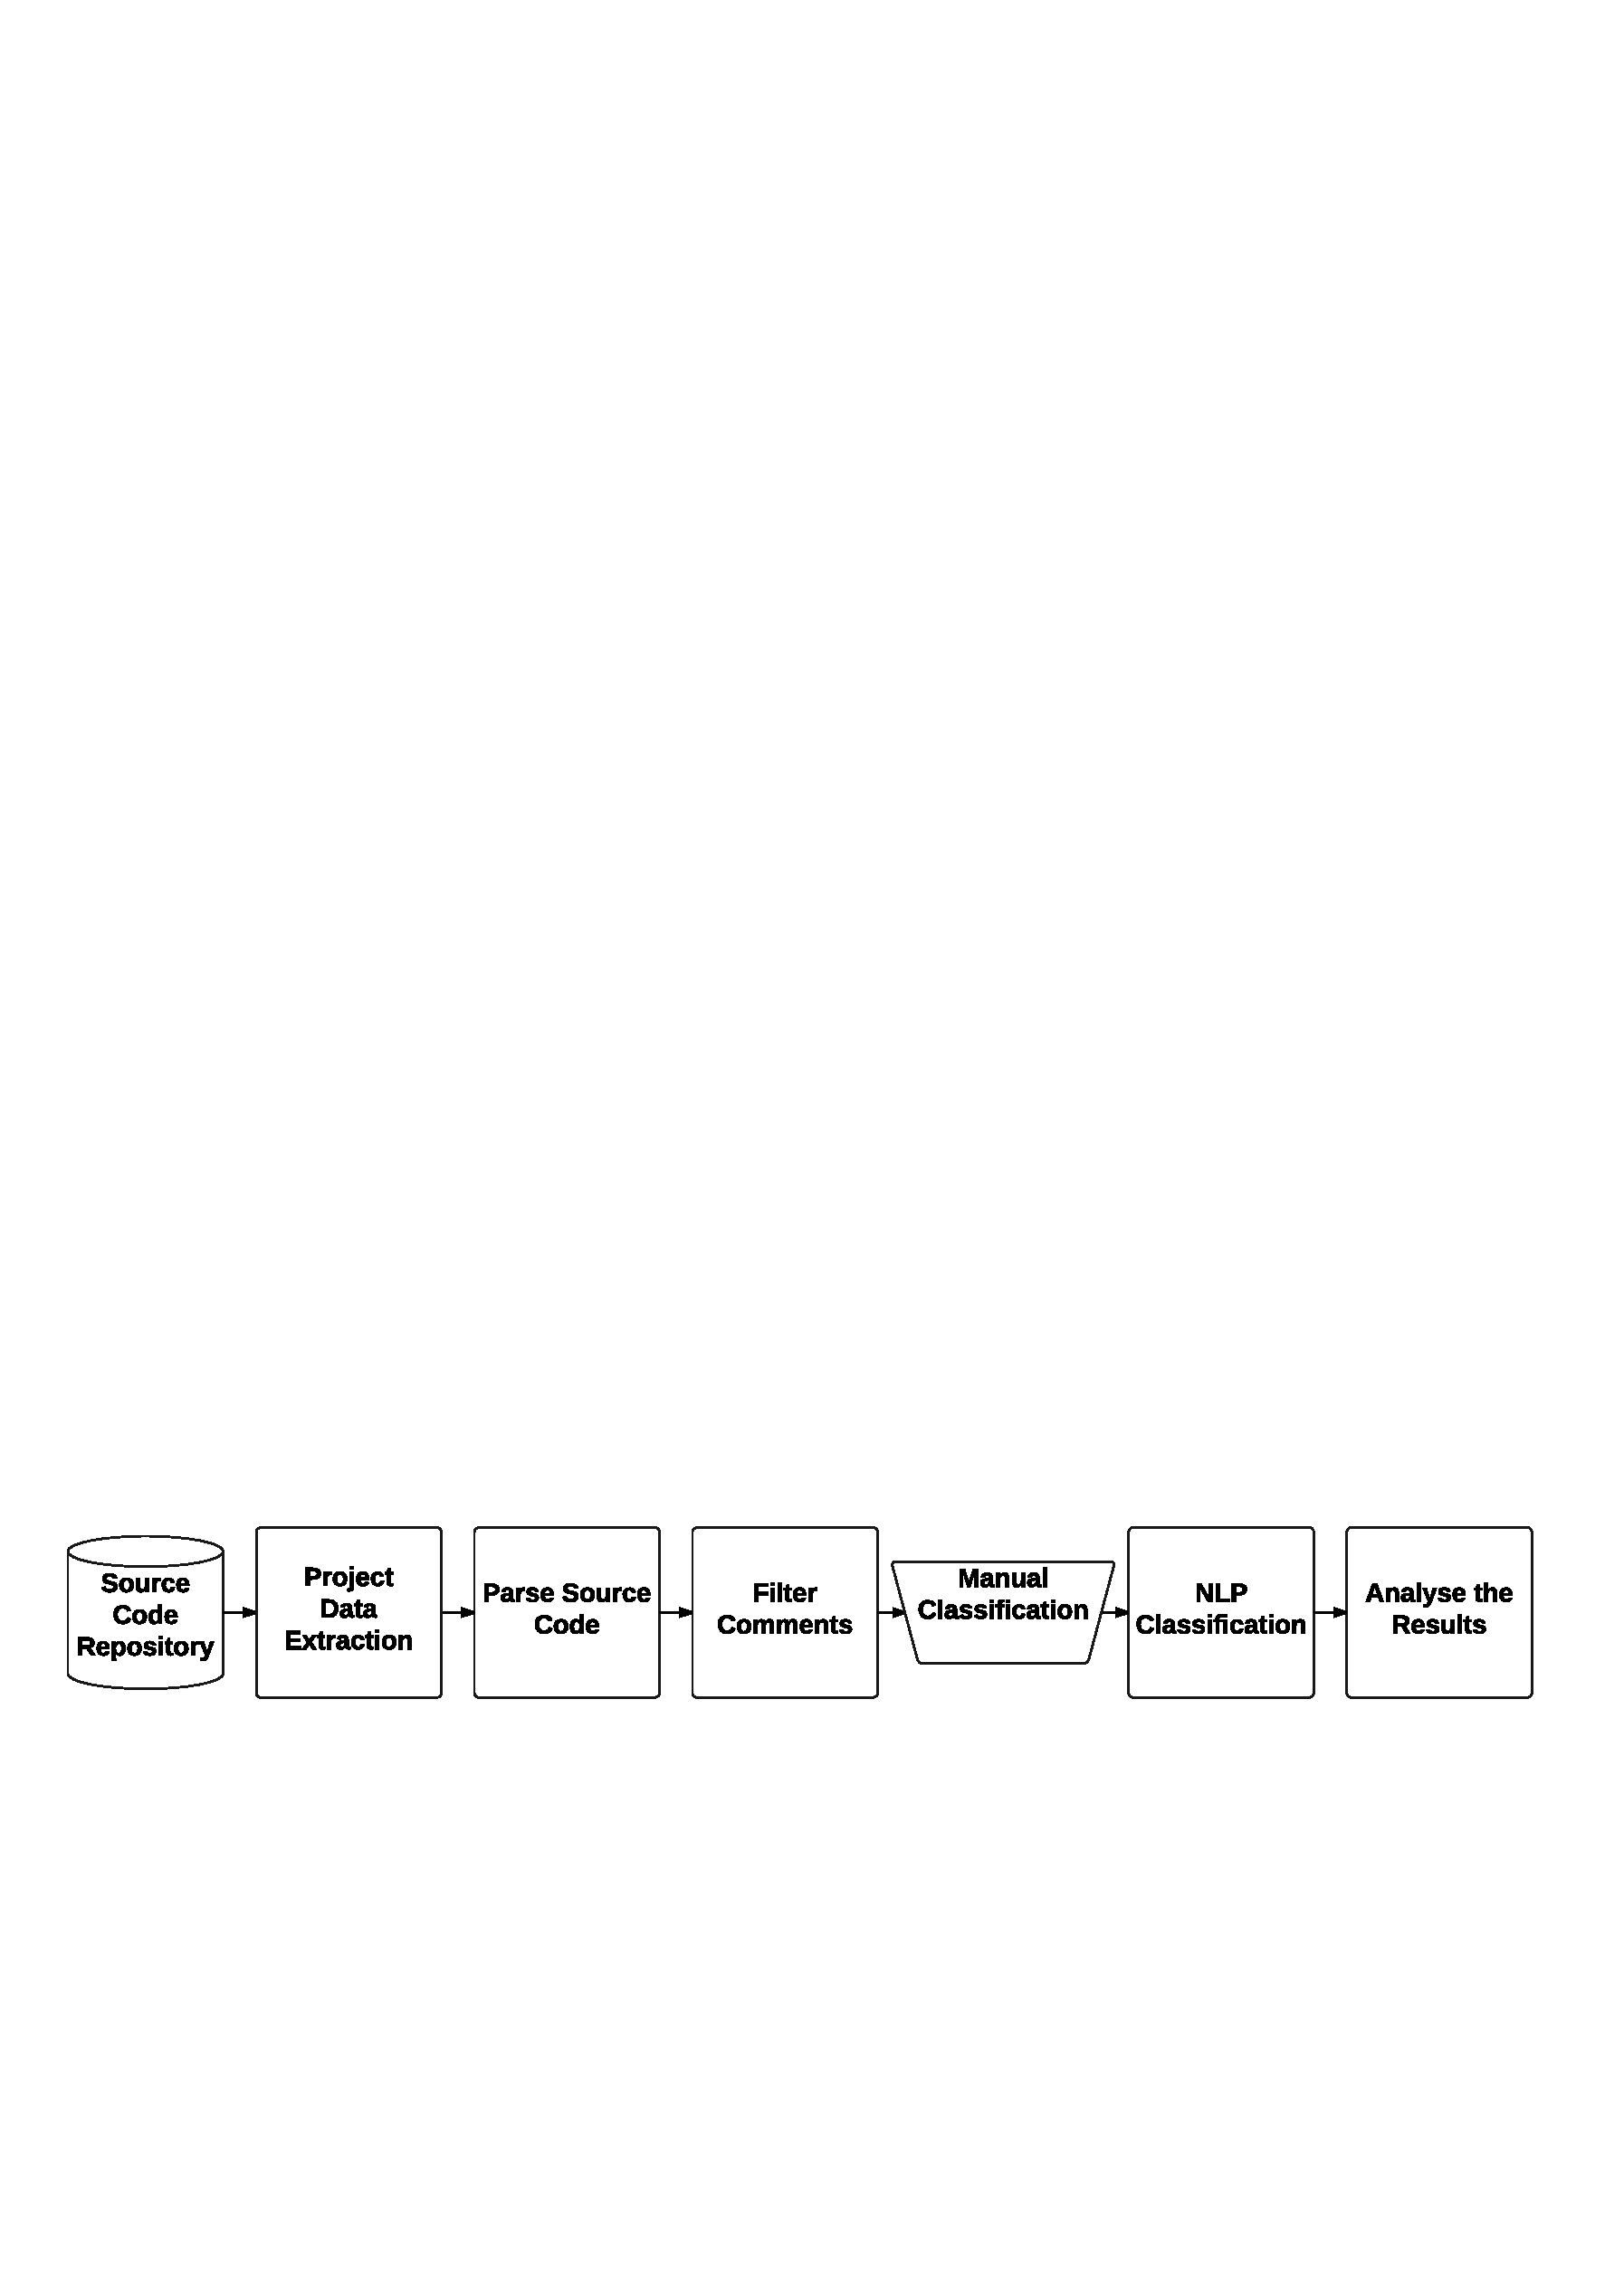
\includegraphics[width=1\textwidth]{figures/approach.pdf}
  \caption{Approach overview}
  \label{fig:approach}
\end{figure*}

The main goal of our study is to effectively identify \SATD. To achieve that, we first extract comments from ten open source projects. Then, we apply four filtering heuristics to remove comments that are irrelevant for the identification of \SATD  (e.g., license comments and commented source code) \cite{Maldonado2015MTD}. Finally, we manually classify the remainder of comments into \SATD types, and use these comments as training data for a maximum entropy classifier. Figure~\ref{fig:approach} shows an overview of our approach, and the following subsections details each step of it.
   
\subsection{Data Extraction} % (fold)
\label{sub:data_extraction}

To perform our study, we extract the source code from ten open source projects, namely Apache Ant, Apache Jmeter, ArgoUML, Columba, EMF, Hibernate, JEdit, JFreeChart, JRuby and SQuirrel. We selected these projects since they belong to different application domains, and vary in size (e.g., SLOC), and in the number of contributors.

Table \ref{tab:project_details} provides statistics about each one of the projects used in our study. We provide details about the release used, the number of classes, the total source lines of code (SLOC), the total extracted comments and the number of contributors. A source line of code contain at least one valid character, which is not a blank space or a source code comment. In our study, we only use the Java files to calculate the SLOC, and to do so, we use the tool SLOCCount \cite{wheeler2004:home}. 

The number of contributors was extracted from OpenHub, an on-line community and public directory that offers analytics, search services and tools for open source software \cite{Openhub:home}. It is important to notice that the number of comments shown for each project does not represent the number of commented lines, but rather the number of individual line, block, and Javadoc comments. In total, we obtained more than \todo{} comments, found in \todo{} Java classes.

\begin{table*}[!tbh]
    \begin{center}
    \label{tab:project_details}
            \begin{tabular}{l| c c r c c | p{2.0in}}
            \toprule
            \textbf{Project}   & \textbf{Release}  & \textbf{\# of classes}   & \textbf{SLOC}    & \textbf{\# of comments}  & \textbf{\# of contributors} & \textbf{Description}\\ \midrule 
            Apache Ant     & 1.7.0    & 1,475 & 115,881 & 21,587 & 74  & A Java library and command-line tool to build Java applications.\\
            ArgoUML        & 0.34     & 2,609 & 176,839 & 67,716 & 87  & An UML modeling tool.\\
            Apache Jmeter  & 2.10     & 1,181 &  81,307 & 20,084 & 33  & An application to measure performance and assert functional behavior.\\
            Columba        & 1.4      & 1,711 & 100,200 & 33,895 & 9   & A desktop email client written in Java.\\
            Hibernate      & 3.3.2 GA & 1,356 & 173,467 & 11,630 & 226 & An Object Relational Mapping framework.\\
            EMF            & 2.4.1    & 1,458 & 228,191 & 25,229 & 30  & Eclipse Modeling Framework.\\
            JEdit          & 4.2      &   800 &  88,583 & 1,6991 & 57  & A light weight text editor.\\
            JFreeChart     & 1.0.19   & 1,065 & 132,296 & 23,474 & 19  & A Java library to display graphics and charts.\\
            SQuirrel       & 3.0.3    & 3,108 & 215,234 & 27,474 & 46  & A graphical SQL client written in Java.\\ 
            JRuby          & 1.4.0    & 1,486 & 150,060 & 11,149 & 328 & Is the implementation of the Ruby language using the Java Virtual Machine.\\ \bottomrule
            
        \end{tabular}
    \end{center}
\end{table*}


% subsection data_extraction (end)
\subsection{Parse Source Code} % (fold)
\label{sub:parse_source_code}

% subsection parse_source_code (end)
\subsection{Filter Comments} % (fold)
\label{sub:filter_comments}

% subsection filtering_comments (end)

% subsection heuristics_to_remove_irrelevant_comments (end)
\subsection{Creating Training Datasets} % (fold)
\label{sub:creating_training_datasets}

% subsection creating_training_datasets (end)
\subsection{Run NLP Classifier} % (fold)
\label{sub:run_nlp_classifier}

% subsection run_nlp_classifier (end)